
\section{Contributions to Driftfusion}
	\epigraph{\textit{\enquote{Wow, this is a gold mine!}}}

	\subsection{Introduction}
		During my 3-month stay in Dr.\ Piers R.\ F.\ Barnes and Prof.\ Jenny Nelson groups in Imperial College London, I utilized and expanded a modelling software developed by Dr.\ Phil Calado, Dr.\ Mohammed Azzouzi, Benjamin Hilton, and Piers R.\ F.\ Barnes.
		As the modelling software had already demonstrated a great descriptive power \cite{Belisle2017,Calado2016,Calado2019}, I implemented a few more characterisation techniques with the objective of reproducing and understanding real-world data.
		The impedance spectroscopy simulation is not included here as it has been treated in \cref{ch:impedance}.
		Driftfusion \cite{Calado2018a,Calado2016} is a time resolved, one dimensional, drift\hyp{}diffusion modelling platform.
		It takes advantage of Matlab \texttt{pdepe} solver for partial differential equations with boundary conditions in time and one spatial dimension.
		%Solve initial-boundary value problems for parabolic-elliptic PDEs in 1-D.
		Currently, it can simulate the electrostatic potential, and the density of electrons, holes and one ionic species at specified depths in a multi\hyp{}layered electronic device and at specified time points.
		Even if an heterojunction version of the code is available, I implemented functions for the homojunction (every material has the same bandgap) release, which is much more stable and tested.
		All the described scripts can be obtained from \url{https://github.com/barnesgroupICL/Driftfusion/tree/2018-EIS}.


	\subsection{Additions to the Driftfusion Core}
		\epigraph{$>>$ 0.1 + 0.2 == 0.3\\
			ans =\\
			logical\\
			0}{MATLAB}



\paragraph{\texttt{equilibrate\_minimal} -- Generate a reduced set of solutions at standard conditions}
It is a reduced version of \texttt{equilibrate}. 
Uses analytical initial conditions and runs to equilibrium and steady state, obtaining just the most important solutions
 Takes the parameters from \texttt{pin\-Params.m} file and tries
 to obtain a steady state solution (as if the device has been left for
 a long period of time). This solution can then be used as accurate
 initial conditions for other simulations, \textsl{e.g.}\ a JV scan.
 Note that the stabilisation time is consistently adjusted to appropriate values for to
 ensure there are numerous mesh points where large gradients in the time
 dimension are present.
 
\textit{Inputs:} optional, struct containing the needed parameters as obtained
     from \texttt{pin\-Params.m}.
     
\textit{Outputs:} \texttt{sol\_eq} - short circuit, dark, no mobile ionic defects, no \gls{srh};
   \texttt{sol\_i\_eq} - short circuit, dark, mobile ionic defects, no \gls{srh};
   \texttt{sol\_i\_eq\_SR} - short circuit, dark, mobile ionic defects, with \gls{srh};
   \texttt{ssol\_i\_eq} - open circuit, dark, mobile ionic defects, no \gls{srh};
   \texttt{ssol\_i\_eq\_SR} - open circuit, dark, mobile ionic defects, with \gls{srh};
   \texttt{sol\_i\_1S\_SR} - short circuit, 1 sun, mobile ionic defects, with \gls{srh};
   \texttt{ssol\_i\_1S\_SR} - open circuit, 1 sun, mobile ionic defects, with \gls{srh}.

\textit{Requires:} \texttt{pin\-drift}, \texttt{pinParams}, \texttt{stabilize}.

\textit{Required by:} \texttt{examples\_unit\_test}.

		\paragraph{\texttt{verify\-Stabilization} -- Verifies if the provided solution has evolved until its steady state}\label{verifyStabilization}
Checks if the solution reached a stabilised (\textsl{i.e.}\ steady state) status comparing the final time point with a manually specified time point. Beware that this can have false positives when the analysed solution had
 has been run over a time which is so small that the ionic movement did not even start.
 For each variable under study, the comparison integrates over the solution thickness the absolute value of the difference in the profile of this variable at two different times in the solution.
 If this integrated difference is larger than \num{1e-4} times the integrated profile of the same variable at the final time point at which its spatially average value has been subtracted, the solution is considered as not stabilised yet.
 The definition of this last threshold, will cause completely flat profiles to be unsuitable for this check.
 The variables which are employed are: ionic density, electrostatic potential, decimal logarithm of electrons density and decimal logarithm of holes density.
 
\textit{Inputs:} 1) a solution matrix, not the full structure, as contained in
     structures created by \texttt{pin\-drift};
   2) the time mesh array, as generated by \texttt{meshgen\_t} and included
     in structures created by \texttt{pin\-drift};
   3) the fraction of final time that can be used as a
     reference. In case of a stabilisation, the smaller the stricter the
     check, for example if a solution has been run over \SI{10}{\s}, and the provided fraction is \num{1e-5}, the script will compare the solution at \SI{0.1}{\us} with the final one at \SI{10}{\s}. In case of a periodic time evolution, a specific value
     corresponding to the previous-to last cycle have to be used. The
     value needs to be strictly between 0 and 1.

\textit{Outputs:} a logic (true/false) asserting if the solution in input reached its stability.

%\textit{Requires:} nothing.

\textit{Required by:} \texttt{CE\_full\_exec}, \texttt{CE\_single\_exec}, \texttt{find\-Optim\-Voc}, \texttt{IS\-wave\_EA\_single\_exec}, \texttt{stabilize}, \texttt{TPV\-const\_full\_exec}, \texttt{TPV\_single\_exec}.

		\paragraph{\texttt{stabilize} -- Evolves a solution until its steady state}
Simulates the solution increasing the maximum time until when steady state is reached. 
\texttt{verify\-Stabilization} is used for checking the reaching of the steady state.
For all the simulations including transients, the stabilisation of the starting solution is of utmost importance.

\textit{Inputs:} 1) a solution structure as created by \texttt{pin\-drift};
   2) optional boolean, true by default, 
     if true forces the simulation to run at least once, if false the
     stabilisation is run just when needed.
     
\textit{Outputs:} a solution structure that reached its steady state.

\textit{Requires:} \texttt{pin\-drift}, \texttt{verify\-Stabilization}.

\textit{Required by:} \texttt{CE\_full\_exec}, \texttt{change\-Light}, \texttt{equilibrate}, \texttt{equilibrate\_minimal}, \texttt{find\-Optim\-Voc}, \texttt{gen\-Int\-Structs\-Real\-Voc}, \texttt{gen\-Vapp\-Structs}, \texttt{ideality\_from\_dark\_jVpoints}, \texttt{IS\-wave\_EA\_single\_exec}, \texttt{IS\-wave\_full\_exec}, \texttt{IS\-wave\_full\_exec\_nonparallel}, \texttt{TPV\_single\_exec}.

		\paragraph{\texttt{asymmetricize} -- Break a symmetrical solution}\label{asymmetricize}
		Break a symmetrical solution (a symmetrical solution it is a repeated \textit{p}-\textit{i}-\textit{n}-\textit{n}-\textit{i}-\textit{p} stack, mainly used for simulating open circuit conditions, so that no boundary condition has to be set for the cathode) in two halves. Has the opposite use of the \texttt{symmetricize} function.
		Please note that further stabilisation could be required.
		
		\textit{Inputs:} a symmetric structure as created by \texttt{pin\-drift} using the OC parameter set to 1.
		
		\textit{Outputs:} an asymmetric structure as created by \texttt{pin\-drift} using the OC
		     parameter set to 0 and applied voltage identical to the open circuit
		     voltage taken from the input symmetric structure.
		     
	\textit{Requires:} \texttt{pin\-drift}
	
	\textit{Required by:} \texttt{CE\_full\_exec}, \texttt{gen\-Int\-Structs\-Real\-Voc}, \texttt{IS\-wave\_full\_exec}, \texttt{IS\-wave\_full\_exec\_nonparallel}, \texttt{EA\_full\_exec}.

		\paragraph{\texttt{change\-Light} -- Change the illumination intensity of a solution}
		Generate solutions at a new light intensity.
		
		\textit{Inputs:} 1) a solution structure as created by \texttt{pin\-drift};
		2) the requested light intensity, zero is not supported as it is
		    much more robust to obtain a dark solution directly from equilibrate;
		3) the initial stabilisation time, can be zero for an automatic
		     guess.
		     
		\textit{Outputs:} a solution structure at the new light intensity.
		
		\textit{Requires:} \texttt{pin\-drift}, \texttt{stabilize}.
		
			\textit{Required by:} \texttt{equilibrate\_minimal}, \texttt{gen\-Int\-Structs}.
			
		\paragraph{\texttt{gen\-Int\-Structs} -- Generates a list of solutions at various light intensities}\label{genIntStructs}
Generates a cell containing structures of solutions at logarithmically spaced light intensities, starting from the one at lower light illumination. Can be used for both symmetrical (for obtaining open circuit solutions) or asymmetrical solutions.

		\textit{Inputs:} 1) a solution structure as created by \texttt{pin\-drift} in dark conditions; 
		2) highest requested illumination;
		3) lowest requested illumination;
		4) number of illumination requested between the lowest and the highest illumination points, including extrema, except dark;
		5) logical, whether to include the dark solution in the output structure
		
\textit{Outputs:} 1) a cell containing structures of solutions at various light
     intensities;
2) an array with the voltages present in the solution, which is
     an approximation of the \gls{voc}, getting populated just if the input
     structures were at open circuit;
 3) an array with the currents present in the solutions.
 
\textit{Requires:} \texttt{change\-Light}, \texttt{pin\-drift}, \texttt{pinana}.

\textit{Required by:} \texttt{examples\_unit\_test}, \texttt{gen\-Int\-Structs\-Real\-Voc}.

		\paragraph{\texttt{gen\-Vapp\-Structs} -- Generates a list of solutions at various applied voltages}\label{genVappStructs}
Generates a cell containing asymmetric structures of solutions at various applied voltages.
Differently from \texttt{gen\-Int\-Structs} case, here the voltage array has to be specified.

\textit{Inputs:} 1) a solution asymmetric struct as created by \texttt{pin\-drift};
2) an array containing the requested applied voltages list.

\textit{Outputs:} a cell containing structures of solutions at various applied
     voltages, ordered with ascending voltages.
     
\textit{Requires:} \texttt{pin\-drift}, \texttt{pinana}, \texttt{stabilize}.

\textit{Required by:} \texttt{examples\_unit\_test}.

		\paragraph{\texttt{find\-Optim\-Voc} -- Find the exact \glsentryshort{voc} minimizing the current output}
Stabilize an asymmetric solution to the real open circuit voltage
which is the applied voltage where the current is minimized,
starting from the voltage present in the given solution. The suggested
workflow is to stabilise a symmetric solution (so that the charges
profile are close to OC conditions) and break in a half with
\texttt{asymmetricize}.
Differently from \texttt{find\-Voc}, this version requires MATLAB's Optimization Toolbox.
While the \gls{voc} can be conveniently obtained from the symmetrical solution, in same cases the zero current condition is not matched.
For this reason, the search for an applied voltage that minimizes the residual current can be needed.
		
		\textit{Inputs:} an asymmetric structure as created by \texttt{pin\-drift}, ideally
    breaking a symmetric solution using \texttt{asymmetricize} function so that
    the starting applied voltage is already close to the real \gls{voc}.
    
\textit{Outputs:} 1) an asymmetric structure as created by \texttt{pin\-drift} using the OC
     parameter set to 0 and applied voltage identical to the real open
     circuit voltage;
2) the value of the obtained open circuit voltage.

\textit{Requires:} \texttt{pin\-drift}, \texttt{pinana}, \texttt{stabilize}.

\textit{Required by:} \texttt{gen\-Int\-Structs\-Real\-Voc}.

		\paragraph{\texttt{gen\-Int\-Structs\-Real\-Voc} -- Generates a list of solutions at various light intensities ensuring open circuit}
		Generates a cell containing structures of asymmetric solutions at various light intensities at an accurate \gls{voc}.
		This script just uses other three scripts: \texttt{gen\-Int\-Structs}, \texttt{find\-Optim\-Voc}
		 and \texttt{asymmetricize}. Both symmetric and asymmetric solutions are supported in input, but the usage of symmetric solutions is strongly encouraged as the \texttt{find\-Optim\-Voc} will start from a condition closer to the \gls{voc}.
		
				\textit{Inputs:} 1) a solution structure as created by \texttt{pin\-drift} in dark
				     conditions, preferably a symmetric (open circuit) solution;
				2) higher requested illumination;
				3) lower requested illumination;
				4) number of requested illumination points between the lowest and the highest illuminations, including extrema, except dark;
				5) logical, whether to include the dark solution in the output
				     structure.
				
		\textit{Outputs:} 1) cell containing structures of asymmetric solutions at various light
		     intensities with an applied voltage equal to the \gls{voc};
		2) an array with the \gls{voc} values.
		
		\textit{Requires:} \texttt{change\-Light}, \texttt{pin\-drift}, \texttt{gen\-Int\-Structs},
		   \texttt{asymmetricize}, \texttt{find\-Optim\-Voc}, \texttt{stabilize}.
		   
%		\textit{Required by:} 
		
		\paragraph{\texttt{from\-Steady\-State\-Struct\-To\-Txt} -- Exports stabilised solutions data to text for plotting externally}
		Save the main data from a stabilised solution created by \texttt{pin\-drift} to text files, using a format easy to import with Origin (from OriginLab).
				\textit{Inputs:} 1) a structure as created by \texttt{pin\-drift};
				2) a char array to be used as prefix for the saved files names.
%		\textit{Outputs:} none.
%		\textit{Requires:} nothing.
%		\textit{Required by:} 

		\paragraph{\texttt{plot\_charges\_single} -- Plots various density and energy profiles over time}
Plot free charges and ions densities, and energy levels over device thickness and over time.
 This is inspired by Dr.\ Phil Calado's \texttt{pinExtract2.m} but rewritten.
 The created graphics include: profiles of net charge density and 
 comparison with the final profile; conduction and valence bands and 
 quasi-Fermi levels profiles; profiles of total concentration of 
 particles densities and comparison with the final profile, divided 
 per particle type; time evolution of voltage, current and specific 
 particles types in specific positions.

		\textit{Inputs:} 1) a symmetric or asymmetric structure of a solution evolving over time;
		2) optional char array, if provided saves the images in the current directory with the name starting with it.
%\textit{Outputs:} 
%\textit{Requires:} 
%\textit{Required by:} 

%	\subsection{Ideality Factor}
			\paragraph{\texttt{ideality\_from\_Voc} -- Obtains ideality factor from voltage \textsl{versus} illumination intensity relation}\label{dd_ideality}
	As explained in \cpageref{characterization_ideality}, the ideality factor can be obtained relating \gls{voc} to the light intensity.
	%		 data of a device illuminated at various illumination intensities
	
			\textit{Inputs:} a cell containing structures at open circuit and various
	     light intensities. The open circuit can be either obtained from
	     symmetric solutions (from \texttt{gen\-Int\-Structs}) or from asymmetric solutions
	     with applied voltage (from \texttt{gen\-Int\-Structs\-Real\-Voc}).
	
	\textit{Outputs:} the numeric ideality factor.
	
	\textit{Requires:} \texttt{pinana}.
	
	\textit{Required by:} \texttt{examples\_unit\_test}.
	
				\paragraph{\texttt{ideality\_from\_dark\_jVpoints} -- Obtains voltage dependent ideality factor from the stabilised current at different voltages}
	A voltage dependent ideality factor can be obtained from a dark current\hyp{}voltage sweep (or stabilised points in the case of hysteretic\index{hysteresis} devices) \cite{Honsberg2019}.
	%		 data of a device illuminated at various illumination intensities
	
	\textit{Inputs:} 1) an asymmetric solution structure as created by \texttt{pin\-drift} in dark conditions;
	2) the maximum voltage point;
	3) the distance between voltage points.
	
	\textit{Outputs:} an array of ideality factor at different applied voltages.
	
	\textit{Requires:} \texttt{pin\-drift}, \texttt{pinana}, \texttt{stabilize}.
	
	\textit{Required by:} \texttt{examples\_unit\_test}.


	\subsection{Charge Extraction}\label{dd_ce}
		Careful stabilisation of illuminated solutions is crucial, especially for avoiding glitches appearing at high light illumination (minority charges accumulation at the edges of the symmetric solution).

		\paragraph{\texttt{CE\_full\_exec} -- Do Charge Extraction in a range of background light intensities}		
		
		\textit{Inputs:} 1) can be a cell structure containing structures at various background light intensities.
			This can be generated using \texttt{gen\-Int\-Structs}.
		    Otherwise it can be a single structure as created by \texttt{pin\-drift};
		   2) logical, whether to graph the individual solutions and
		     the overall graphics;
		   3) logical, whether to assign in volatile base
		     workspace the calculated solutions of single CE decays.
		
		\textit{Outputs:} a structure containing the most important results of the simulation.
		
		\textit{Requires:} \texttt{CE\_single\_exec}, \texttt{CE\_ISstep\_single\_analysis},   \texttt{CE\_ISstep\_subtracting\_analysis}, \texttt{CE\_full\_fit}, \texttt{CE\_full\_analysis},  \texttt{asymmetricize}, \texttt{pinana}.
		
%		\textit{Required by:} \texttt{}.


\paragraph{\texttt{CE\_single\_exec} -- Do a single Charge Extraction experiment}		

\textit{Inputs:} 1) a single asymmetric structure as created by \texttt{pin\-drift};
2) a first guess for maximum time which should be enough for registering the full extraction.

\textit{Outputs:} a structure with a solution evolving after the start of the CE experiment.

\textit{Requires:} \texttt{pin\-drift}, \texttt{verify\-Stabilization}.

\textit{Required by:} \texttt{CE\_full\_exec}.


		\paragraph{\texttt{CE\_full\_analysis} -- Plot Charge Extraction in a range of background light intensity \textsl{versus} open circuit voltage}


\textit{Inputs:} a structure containing the most important results of the CE simulation.

%		\textit{Outputs:} .

%		\textit{Requires:} \texttt{}.

\textit{Required by:} \texttt{CE\_full\_exec}.


		\paragraph{\texttt{CE\_full\_fit} -- Calculate geometric and chemical capacitance\index{chemical capacitance} from CE data}		
		
		\textit{Inputs:} 1) an array containing the voltage drops which were
		     imposed in the CE experiments. As usually the CE experiments goes from
		     open circuit to short circuit, the voltage drop is equal to the \gls{voc};
		   2) an array with the extracted charges from CE at various light
		     intensities.
		
		\textit{Outputs:} an array with the values from the linear + exponential fit:
		     linear gradient, exponential function linear factor, exponent.
		
%		\textit{Requires:} \texttt{}.
		
		\textit{Required by:} \texttt{CE\_full\_exec}.
		
		\paragraph{\texttt{CE\_ISstep\_single\_analysis} -- Calculate charge extracted by Charge Extraction integrating the current}		
		
		\textit{Inputs:} 1) a structure with a solution being perturbed by CE;
		   2) original light intensity is needed in input as the solution provided
		     in input for CE is in dark;
		   3) logical, whether the residual current should
		     be subtracted, usually false for CE;
		   4) logical, whether to calculate the ionic contribution and graph the solution.
		
		\textit{Outputs:} 1) array of cumulative charge extracted at each time point;
		2) index of the previous array indicating the end of the early extraction, time at which the electronic charge have been extracted but the ionic defects did not move yet.
		
%		\textit{Requires:} \texttt{}.
		
		\textit{Required by:} \texttt{CE\_full\_exec}.
		
		\paragraph{\texttt{CE\_ISstep\_subtracting\_analysis} -- Calculate the charge excess in device under illumination}
			The carriers density profile in the illuminated steady state solution is subtracted from the profiles
			 at all time points of the solution evolving during the charge extraction experiment.
			 These profiles are integrated over the device thickness, obtaining a time resolved excess charge amount.
			This is used as a reference for Charge Extraction.
		
		\textit{Inputs:} 1) structure of the stable solution before the CE experiment, to be used as a reference;
		2) structure of the solution perturbed by CE.
		
		\textit{Outputs:} 1) array of excess charges in the whole device versus time;
		2) array of excess charges in the intrinsic layer versus time.
		
%		\textit{Requires:} \texttt{}.
		\textit{Required by:} \texttt{CE\_full\_exec}.
		

	\subsection{Transient PhotoVoltage}\label{dd_tpv}

		\paragraph{\texttt{TPV\-const\_full\_exec} -- Simulate Transient PhotoVoltage in a range of background light intensities without varying the pulse intensity}	
The pulse intensity is tuned to be a small perturbation compared to the 1
 sun background illumination, then the \acr{tpv} is simulated for all the
 provided solutions without changing the chosen pulse intensity.
 
		\textit{Inputs:} 1) can be a cell structure containing structures at various background
		     light intensities. This can be generated using \texttt{gen\-Int\-Structs}.
		     Otherwise it can be a single structure as created by \texttt{pin\-drift};
		   2) logical, whether to assign in volatile base
		     workspace the calculated solutions of single \acr{tpv} decays.
				
		\textit{Outputs:} a structure containing the most important results of the simulation.
		
		\textit{Requires:} \texttt{TPV\_single\_exec}, \texttt{TPV\_single\_analysis}.
		
%		\textit{Required by:} \texttt{}.
		
		
				\paragraph{\texttt{TPV\-variab\_full\_exec} -- Simulate Transient PhotoVoltage in a range of background light intensities adapting the pulse intensity for each simulation}
				For each of the provided solutions, the pulse intensity is tuned to be a small perturbation compared to the background illumination intensity, then the \acr{tpv} is simulated.
				
				\textit{Inputs:} 1) can be a cell structure containing structures at various background
				light intensities. This can be generated using \texttt{gen\-Int\-Structs}.
				Otherwise it can be a single struct as created by \texttt{pin\-drift};
				2) logical, whether to assign in volatile base
				workspace the calculated solutions of single \acr{tpv} decays.
				
				\textit{Outputs:} a structure containing the most important results of the simulation.
				
				\textit{Requires:} \texttt{TPV\_single\_exec}, \texttt{TPV\_single\_analysis}.
		
		
		\paragraph{\texttt{TPV\_single\_exec} -- Perform a single TPV simulation}
		
		\textit{Inputs:} 1) a single symmetric (\textsl{i.e.}\ open circuit) structure as created by \texttt{pin\-drift};
		2) a first guess for maximum time which should be enough for simulating the full decay, if zero is provided a value of \SI{1e-5}{\s} is used and no further exploration of the simulation time is performed (this is useful when we are just interested in the amount of voltage variation, rather than in the full decay);
		3) intensity of the perturbing light pulse.
		
		\textit{Outputs:} a structure with a solution being perturbed by a light pulse.
		
		\textit{Requires:} \texttt{pin\-drift}, \texttt{verify\-Stabilization}.
		
		\textit{Required by:} \texttt{TPV\-const\_full\_exec}, \texttt{TPV\-variab\_full\_exec}.
		
		

		
%		\textit{Required by:} \texttt{}.
		
		\paragraph{\texttt{TPV\_full\_analysis} -- Plot TPV}
			Both mono and bi exponential fitting results are plotted \textsl{versus} light-bias.
			
				\textit{Inputs:} a structure containing the most important results of the \acr{tpv} simulation.
		
%		\textit{Outputs:} .
		
%		\textit{Requires:} \texttt{}.
		
		\textit{Required by:} \texttt{TPV\-const\_full\_exec}, \texttt{TPV\-variab\_full\_exec}.
		
		\paragraph{\texttt{TPV\_single\_analysis} -- Fit voltage decays from single TPV solutions using MultiStart and do graphics}
		Fit the voltage \textsl{versus} time profile of the provided perturbed solution with a mono\hyp{}exponential and a bi\hyp{}exponential formula.
		Use Matlab's MultiStart from Global Optimization Toolbox in order to find the best bi\hyp{}exponential fitting avoiding local minima.
		An initial guess from a previous fitting can be provided in input.
		
		\textit{Inputs:} 1) a structure with a solution being perturbed by a light pulse;
		2) optional, initial guess for linear factor of fast decay of bi-exponential fit;
		3) optional, initial guess for lifetime of fast decay of bi-exponential fit;
		4) optional, initial guess for linear factor of slow decay of bi-exponential fit;
		5) optional, initial guess for lifetime of slow decay of bi-exponential fit.
		
		\textit{Outputs:} 1) steady state voltage being present before the pulse;
		   2) maximum voltage variation due to the pulse;
		   3) linear factor of mono-exponential fit;
		   4) lifetime of mono-exponential fit;
		   5) linear factor of fast decay of bi-exponential fit;
		   6) lifetime of fast decay of bi-exponential fit;
		   7) linear factor of slow decay of bi-exponential fit;
		   8) lifetime of slow decay of bi-exponential fit.
		
%		\textit{Requires:} \texttt{}.
		
		\textit{Required by:} \texttt{TPV\-const\_full\_exec}, \texttt{TPV\-variab\_full\_exec}.
		
		\paragraph{\texttt{TPV\_single\_analysis\_noMulti\-Start} -- Fit voltage decays from single TPV solutions and do graphics}
		Fit the voltage \textsl{versus} time profile of the provided perturbed solution with a mono\hyp{}exponential and a bi\hyp{}exponential formula.
		Try various starting point for helping the convergence of bi\hyp{}exponential fitting.
		An initial guess from a previous fitting can be provided in input.
		
		\textit{Inputs:} 1) a structure with a solution being perturbed by a light pulse;
2) optional, initial guess for linear factor of fast decay of bi-exponential fit;
3) optional, initial guess for lifetime of fast decay of bi-exponential fit;
4) optional, initial guess for linear factor of slow decay of bi-exponential fit;
5) optional, initial guess for lifetime of slow decay of bi-exponential fit.

\textit{Outputs:} 1) steady state voltage being present before the pulse;
2) maximum voltage variation due to the pulse;
3) linear factor of mono-exponential fit;
4) lifetime of mono-exponential fit;
5) linear factor of fast decay of bi-exponential fit;
6) lifetime of fast decay of bi-exponential fit;
7) linear factor of slow decay of bi-exponential fit;
8) lifetime of slow decay of bi-exponential fit.
		
%		\textit{Required by:} \texttt{}.
		
		%
		%
		%\subsection{Impedance Spectroscopy in Time Domain}
		%\epigraph{\textit{"I thought you could implement this"\\"Ehm\dots Do you mean\dots by tomorrow?"\\"That would be amazing!"}}
		%
		%\subsection{Impedance Spectroscopy in Frequency Domain}




	\subsection{ElectroAbsorption}\label{software_electroabsorbance}
		\epigraph{First Law of Software Quality:\\
			errors = more code\textsuperscript{2}\\
			$e=mc^2$}

The public release of these routines is waiting for the publication of the related work.
We refer to ElectroAbsorption or Stark spectroscopy as the study of the dependency of the absorbance on the oscillating voltage applied on a complete device with semi\hyp{}transparent electrodes, caused by Franz\hyp{}Keldysh effect.
We simulate the whole $p$-$i$-$n$ stack but consider the absorption just in the intrinsic layer.
Clearly, the Stark effect has to be evaluated locally at any position through the perovskite layer.
The attention has been focussed on the first and the second harmonic effects, respectively with the same and the double frequency as the applied voltage.
The first harmonic component is driven by the product of the steady state electric field $E_|DC|(x)$ and the amplitude of the first harmonic of the oscillating electric field $|E_|AC||$ at each spatial point.
The second harmonic component is related to the square of the oscillating electric field amplitude $|E_|AC|^2|$ at each spatial point.
Thanks to the modularity of the developed routines, some of the functions coded for the impedance spectroscopy modelling are called by ElectroAbsorption routines, specifically: \texttt{IS\-wave\_EA\_single\_fit}, \texttt{IS\-wave\_EA\_single\_demodulation}, and \texttt{IS\-wave\_EA\_single\_exec}.

%		photo induced absorption stark spectroscopy on perovskite solar cells \cite{Roiati2014,Li2016}


\paragraph{\texttt{EA\_full\_exec} -- Perform ElectroAbsorption simulation on all the provided solutions}
Similarly to the impedance simulation performed with \texttt{IS\-wave\_full\_exec}, this routine applies an oscillating voltage on all the provided solutions.
One relevant difference is the fact that the current calculation is disabled, making the analysis faster.
If Matlab's Parallel Computing Toolbox is available, this scripts runs in parallel on all the available physical CPU cores, otherwise it just runs on one core.

\textit{Inputs:} 1) can be a cell structure containing structures at various background
light intensities. This can be generated using \texttt{gen\-Int\-Structs}.
Otherwise it can be a single structure as created by \texttt{pin\-drift};
2) higher frequency limit;
3) lower frequency limit;
4) number of frequency points to simulate;
5) voltage oscillation amplitude in volts, one mV should be enough;
6) logical, after stabilisation sets the mobility of
ionic defects to zero;
7) logical, whether to graph the individual solutions and
the overall graphics.

\textit{Outputs:} a structure containing the most important results of the simulation.

\textit{Requires:} \texttt{asymmetricize}, \texttt{IS\-wave\_EA\_single\_exec},
\texttt{EA\_single\_analysis}, \texttt{EA\_full\_analysis\_phase}, \texttt{pinana}, \texttt{EA\_full\_analysis\_Efield}.

%		\textit{Required by:} \texttt{}.

\paragraph{\texttt{EA\_single\_analysis} -- Calculate ElectroAbsorbance and phase}
The first and second harmonics are locally calculated and averaged over the device thickness.

\textit{Inputs:} 1) a structure where a solution has been perturbed by an
oscillating voltage, as generated from \texttt{IS\-wave\_EA\_single\_exec};
2) logical, when true graphics does not get created, useful when
launched under parallelization (where graphics does not work anyway);
3) logical, whether to fit the position resolved data;
4) logical, get phase \textsl{via} demodulation instead of using a fitting;
5) string, set the directory where to save \texttt{.fig} and \texttt{.png}
image files for second harmonic versus position.
To save in the current directory set the dot directory \texttt{"."}.
To disable saving set \texttt{"missing"} value.

\textit{Outputs:} 1) an array of bias, amplitude and phase of the first
harmonic;
2) a matrix of bias, amplitude and phase of the first
harmonic, each column is a space point;
3) an array of bias, amplitude and phase of the first
harmonic for ionic profile;
4) a matrix of bias, amplitude and phase of the first
harmonic for ionic profile, each column is a space point;
5) an array of bias, amplitude and phase of the second
harmonic;
6) a matrix of bias, amplitude and phase of the second
harmonic, each column is a space point;
7) an array of bias, amplitude and phase of the second
harmonic for ionic profile;
8) a matrix of bias, amplitude and phase of the second
harmonic for ionic profile, each column is a space point;
9) the value of the average squared amplitude of the
AC electric field. It would be identical to the amplitude of the
second harmonic if the contributions from each spatial point was in
phase;
10) a matrix of bias, amplitude and phase of the AC electric
field, each column is a space point.

\textit{Requires:} \texttt{IS\-wave\_EA\_single\_fit}, \texttt{IS\-wave\_EA\_single\_demodulation}.

\textit{Required by:} \texttt{EA\_full\_exec}.



		\paragraph{\texttt{EA\_full\_analysis\_Efield} -- Plot electric field amplitude from ElectroAbsorption in a range of background light intensities or applied DC voltages}
		The amplitude of the spatially averaged electric field first harmonic $(x_2-x_1)^-1 \int_{x_1}{x_2}E_|DC|(x) \cdot E_|AC|(x) \dd x$ and second harmonic $(x_2-x_1)^-1 \int_{x_1}{x_2} E_|AC|^2(x) \dd x$ are plotted \textsl{versus} the applied voltage frequency.
		
				\textit{Inputs:} a structure containing the most important results of the EA simulation.
		
%		\textit{Outputs:} .
		
%		\textit{Requires:} \texttt{}.
		
		\textit{Required by:} \texttt{EA\_full\_exec}.
		
		
		\paragraph{\texttt{EA\_full\_analysis\_phase} -- Plot phase Bode plots from EA in a range of background light intensities or applied DC voltages}
		Plots the first and second harmonic phase shift with regards to the applied voltage.
		
		\textit{Inputs:} a structure containing the most important results of the EA simulation.
		
%		\textit{Outputs:} .
		
%		\textit{Requires:} \texttt{}.
		
		\textit{Required by:} \texttt{EA\_full\_exec}.
		

%		\subsection{Techniques Which Could Be Implemented}
%		\paragraph{IMVS}
%		\paragraph{IMPS}
%		\paragraph{Mott-Schottky}
		%\url{https://en.wikipedia.org/wiki/Mott-Schottky_plot}
		%mott-schottky in organics under illumination 10.1103/PhysRevApplied.7.034018
		%impedance and mott-schottky article in osc \cite{Brus2016}		
		%dyakonov sobre mott-shottky 10.1021/acsaem.8b01119




%\pagebreak[2]
\newpage
\mysection[PyPV]{PyPV: An easy Current-Voltage curves acquisition interface}
	\epigraph{\textit{\enquote{So this bug is 7 years old, right? Why nobody tried to fix it?}}}

	\subsection{Introduction}
		The route to a reliable and efficient device is inevitably a long iterative process.
		In each optimization step a device is fabricated, measured, and the design modified for the next step.
		Part of the evaluation is just a repetitive process which can be automatized without any loss.
		Current-voltage sweeps is the most frequently employed characterisation technique for solar cells, for this reason a fast and easy data acquisition software has been developed.
		The complete software can be downloaded from \url{https://github.com/ilario/PyPV}.

		\begin{SCfigure}%[!hbtp]%
			\centering
			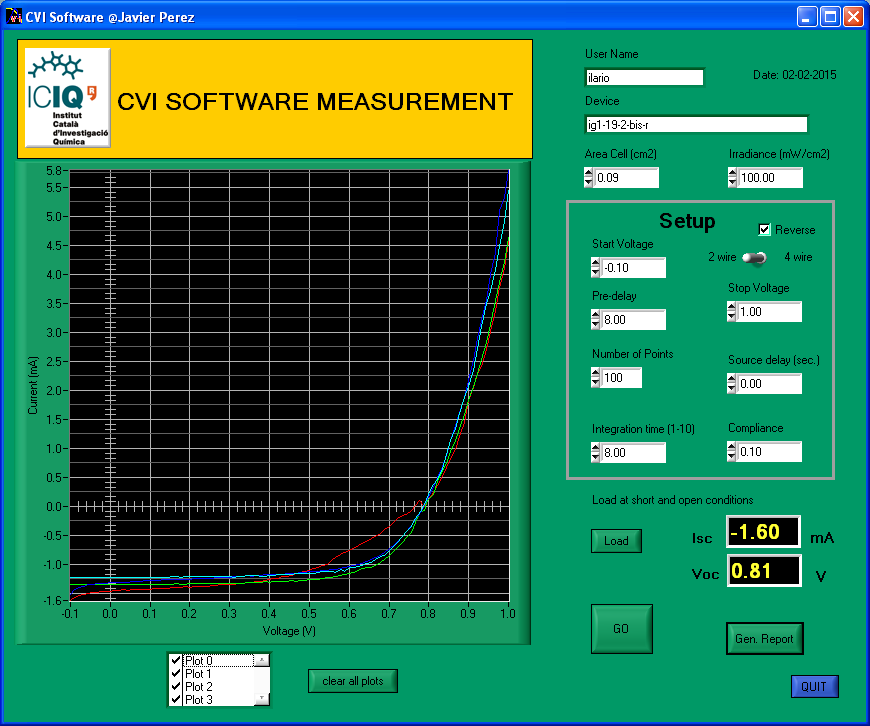
\includegraphics[width=0.7\textwidth]{old_iv_software/old_iv_software.png}
			\mycaption[Legacy software for current-voltage sweep measurement.]{}\label{fig:old_iv_software}
		\end{SCfigure}

		\paragraph{History of the project}
		As a proof of concept, Dr.\ Daniel Fernandez Pinto developed in 2015 a Python library and a small \gls{gui} for communicating with Tektronix Keithley 2400 equipment \textsl{via} NI-VISA \cite{NationalInstruments2019} and running basic operations like current\hyp{}voltage sweeps.
		I went on adding functions and expanding the \gls{gui} until obtaining a fully functional alternative to the legacy LabView software shown in \cref{fig:old_iv_software}.
		In comparison to the mentioned legacy software, PyPV has the advantage of not needing any commercial license which allowed us to use it on various computers.
		Additionally some of the features which will be described below were just missing in the previous software.
		As far as I know, PyPV is currently used in the following research institutions: ICIQ (Institut Català d’Investigació Química), URV (Universitat Rovira i Vrigili), İzmir Katip Çelebi Üniversitesi, and Karamanoglu Mehmetbey University.

		%I received a proof-of-concept software developed by  and decided to continue the development. At that point the software had an interface with few buttons and a working Keithley communication library.

		\paragraph{User's requests}
		The feedback from the new users of the software helped me improving PyPV with the following features: solar simulator shutter control, more robust connection to the GPIB-USB-HS adapter, better installation instructions.

	\subsection{Implementation}
		\epigraph{\textit{\enquote{Ok, I finally completed it, by the way, why did you start developing this?}\\\enquote{Well, it was just a proof of concept, but it's nice you worked on it}}}
		
				\paragraph{Coding language}
				Python~2, rather than the most recent Python~3, has been chosen for the software development.
				This apparently stupid choice was motivated by the requirement of running the software on the obsolete Windows~XP machines still used for the data acquisition.
				Anyway, the usage of Python has two paramount advantages: it can be used without the need of commercial licenses (which was not the case for the previous software relying on LabView) and it is one of the most popular and easy to read coding languages, which will help the future development by other researchers.
				In order to further ease the future development, PEP8 coding style guide was respected \cite{Rossum2017}.
				
				\paragraph{Files structure}
				The software is distributed with the following files:
				\begin{itemize}
					\item \texttt{PyPV.py} -- launcher;
					\item \texttt{mainwindow.py} -- main file where quite everything happens;
					\item \texttt{Keithley2400.py} -- library for communicating with the hardware;
					\item \texttt{VICurves.py} -- where the parameters are extracted from the raw data;
					\item \texttt{mainwindow.ui} -- Qt4 graphical interface.
				\end{itemize}
				
				\paragraph{\Glsentryshort{voc} and \glsentryshort{jsc} estimation}
				The data point respectively closer to zero current or to zero voltage is taken as a first rough approximation.
				Then, the preceding and following 3 data points are selected, if available.
				The set of 7 data points is fitted with a parabolic curve and the final \gls{voc} and \gls{jsc} values are obtained from the result of the fit.
				
				\paragraph{\Glsentryshort{pce} estimation}
				Instead, for obtaining the maximum power point no fitting is performed and the data point having the maximum $J\cdot V$ value is returned.
				From this point and the aforementioned \gls{voc} and \gls{jsc} points, the fill factor is calculated (see \cpageref{characterization_ff}).
				
				\paragraph{Series and shunt resistances}
				The resistances estimation from current\hyp{}voltage sweeps have been implemented but should not be considered for measurements on hysteretic\index{hysteresis} devices, as explained in \cpageref{resistances}.
				Series resistance is obtained from a linear fit of 6 current points at the highest applied voltage and should be taken in consideration just for measurements in dark \cite{Pysch2007}.
				In order to avoid including points affected by the compliance limit, a check of strict monotonicity for the considered current points is included.
				Shunt resistance is obtained from the linear fit of 12 current points close to zero applied voltage, if available.
				
				
		\subsection{User interface}
		
		\begin{sidewaysfigure}
								\centering
			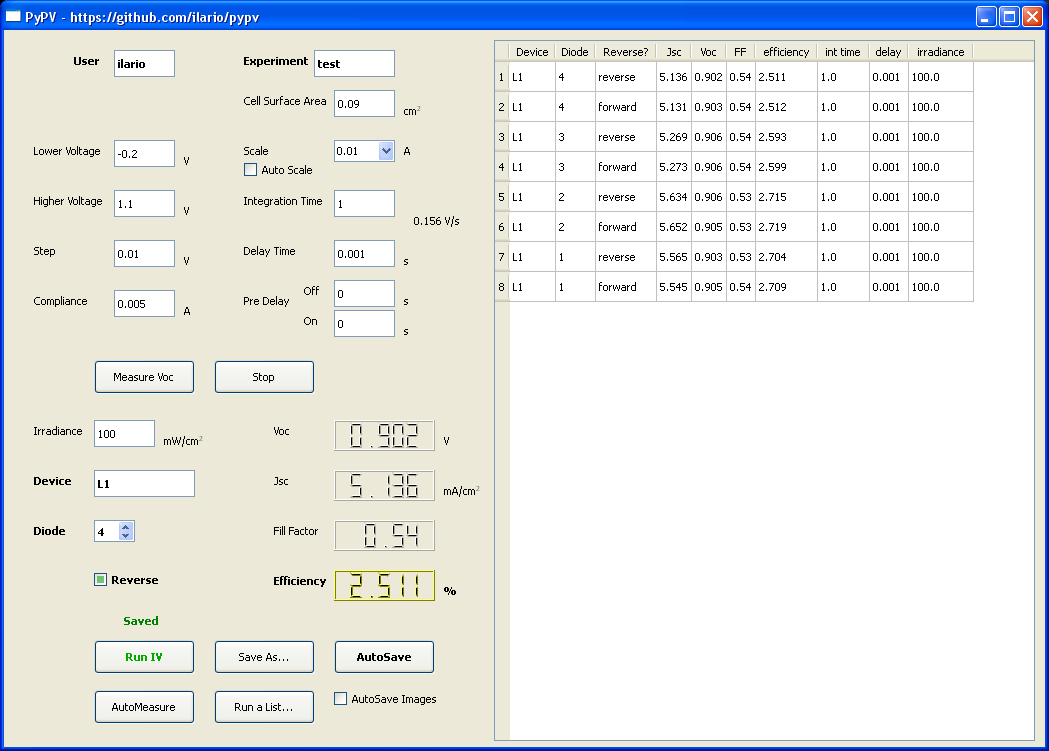
\includegraphics[width=0.9\textwidth]{PyPV/pypv-gui.png}
			\mycaption[PyPV graphical user interface.]{}\label{fig:pypv-gui}
		\end{sidewaysfigure}

		\paragraph{Organisation of the main user interface}
		The components of the graphical user interface are organised with the following order (from top left to bottom right):
		\begin{itemize}
			\item user and experiment identification;
			\item experiment setup;
			\item quick screening buttons;
			\item sample identification and single measurement setup;
			\item single measurement output;
			\item measurement buttons;
			\item saved measurements log, from newest to oldest.
		\end{itemize}
		
		
		\paragraph{User and experiment identification data}
		The user name is prompted, this will be stored in the savings header and, if the "AutoSave" or "AutoMeasure" function is used, a directory named after the user name will be created.
		The experiment codename is prompted for being prepended in the savings suggested and automatic filenames.
		The active area is also prompted at this point.

		\paragraph{Voltage range and step}
		Then, the lowest and highest voltage limits (\textsl{i.e.}\ \texttt{:SOURce:\-VOLTage:\-STARt} or \texttt{:SOURce:\-VOLTage:\-STOP}) are prompted, together with the voltage step (\textsl{i.e.} \texttt{:SOURce:\-VOLTage:\-STEP}).
		The number of measured points (used for the buffer size in \texttt{:TRACe:\-POINts} and for the trigger count in \texttt{:TRIGger:\-COUNt}) can be calculated dividing the voltage range by the voltage step.
		
		\paragraph{Compliance}
		This introduces a maximum limit to the current that can flow in the connected device, in order to avoid overheating and related damages to the solar cell.
		In order to respect this limit, Keithley equipment reduces the applied voltage (this does not get reflected in the saved output, where the capped regions appears simply as a plateau).
		The compliance value (\textsl{i.e.}\ \texttt{:SENSe:\-CURRent:\-PROTection}) has to be smaller than the chosen scale.
		
		\paragraph{Scale and "Auto Scale"}
		As it was explained in \cpageref{autoscale}, the "automatic scale" feature of the Keithley is detrimental for perovskite solar cells dynamic (like a current\hyp{}voltage sweep) measurements.
		For this reason a check and a combo box have been added for enabling\-/disabling automatic scale and setting the manual scale (\textsl{i.e.}\ \texttt{:SOURce:\-CURRent:\-RANGe}).
		
		\paragraph{Integration time, delay time, and scan speed calculation}
		Integration time (\textsl{i.e.}\ \texttt{:SENSe:\-VOLTage:\-NPLCycles}) is the number of power line cycles during which each current point is measured \cite{KeithleyInstruments2011}.
		For example, on a \SI{50}{\Hz} electrical network, an integration time of 1 means that the current is measured during \SI{20}{\ms} for each voltage point.
		Delay time (\textsl{i.e.}\ \texttt{:SOURce:\-DELay}) is the time waited for the current stabilisation after the voltage step.
The scan speed $s[V/s]$ is obtained from the voltage step \texttt{:SENSe:\-VOLTage:\-STEP} $V_|step|[V]$, integration time $i$ and the delay time \texttt{:SOURce:\-DELay} $t_|delay|[s]$ Keithley's parameters with the following \textit{empirical} expression estimated by Werther Cambarau:

\begin{equation}
s = \frac{V_|step|}{0.003 + t_|delay| + 0.06 \cdot i}
\end{equation}

where $t_|delay|$ is \SI{1}{\ms} for our measurement conditions.

\paragraph{Shutter control}
If the employed solar simulator has a remotely controlled shutter, this should be possible to connect to the RS-232 serial port on Keithley.
Two parameters control the opening and closing of the illumination shutter: "pre-delay off" and "pre-delay on".
The former indicates how long the illumination should be off, after this, the shutter gets opened and the latter time is waited before running the sweep.
The off time is mainly useful when using the "AutoMeasure" feature, which will be mentioned further in the text.
During all these steps, the device is kept at open circuit.
If the parameters are set to zero, the shutter control is disabled.

\paragraph{Quick screening buttons}
Open circuit voltage real time measurement is available.
This helps the user to have a quick idea of which diodes are worth measuring.

\paragraph{Irradiance, device and diode identification, scan direction}
Here the user can find the parameters which most likely will vary within an experiment: the illumination intensity, the device identification string (substrate codename), the identification number of the diode in the substrate (with a numeric up-down, in case there are more than one, see \cref{fig:device}), and the sweep scan direction (with a check box, see \cpageref{characterization_fwdrev}).

\paragraph{Latest measured parameters output}
At the end of each measurement, the calculated performance parameters are printed in four large boxes.

\paragraph{Unsaved results indicator}
Just after each measurement, a red "Not saved" text remembers to the user that the data needs to be saved, or it will be lost when the next measurement is performed.
A green "Saved" text confirms to the user that the latest measurement has been saved.

\paragraph{"Run IV" button}
After closing and opening the illumination shutter, it starts a single current\hyp{}voltage scan, then updates the parameters shown in the large boxes and spawns a plot window like the one in \cref{fig:pypv-plot}.

\begin{SCfigure}
	\centering
	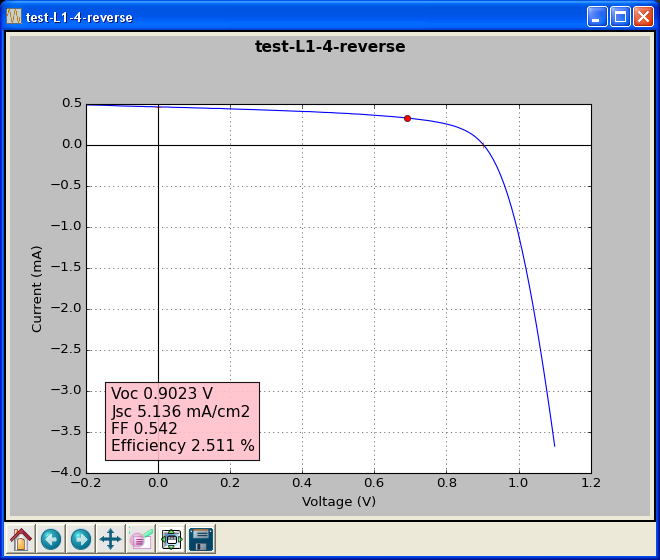
\includegraphics[width=0.7\textwidth]{PyPV/pypv-plot.png}
	\mycaption[Current\hyp{}voltage plot window of PyPV\@.]{
		The plot window includes the main performance data and can be manually resized, zoomed, and saved as an image.
	}\label{fig:pypv-plot}
\end{SCfigure}

\paragraph{"Save As\dots" button}
Opens a prompt for choosing the saving directory and file name.
A suggested file name is provided, as described in \cpageref{pypv_naming_files}, but can be changed.
This also adds a line in the saved measurements table on the right side of \gls{gui}.

\paragraph{"AutoSave" button}
Alike the "Save As\dots" button but it directly employs the directory and the file name obtained from the user name, date, experiment codename, device codename, diode number, illumination intensity, and scan direction as described in \cpageref{pypv_naming_directories,pypv_naming_files}.
Then adds an entry in the saved measurements table.
If the "AutoSave Images" check is active, this also saves a PNG image of the plot in the same directory and with the same base name as the text file but with extension \texttt{.png}.

\paragraph{"Run a List\dots" button}
This function allows the user to select a CSV file in which a series of measurements is specified and runs all of these required sweeps.
This can be used for saving time in setting up every day the same set of measurements.

\paragraph{"AutoMeasure" button}\label{automeasure}
This runs a pre-defined list of sweeps, like the "Run a List\dots" functions but without asking for an input file.
Currently, the measurement steps for AutoMeasure is hard-coded in \texttt{main\-window.py} file.
Hopefully I will change this feature to relay on an external file, like for the aforementioned "Run a List\dots" button.
In the current configuration, the measurement procedure is: 
%the device is kept under illumination at open circuit conditions, then a reverse sweep is measured and, immediately after this, the forward sweep is measured.
\begin{enumerate}
	\item tells the user (using Keithley's display and buzzer) to select the diode number 1 in the device under measurement;
	\item after waiting for the shutter delays, the illumination shutter is opened;
	\item the steady state \gls{voc} is measured;
	\item a reverse sweep is measured from \gls{voc}~+~\SI{0.2}{\V} to the lowest voltage set in the \gls{gui} (the highest voltage setting is ignored);
	\item a plot window is spawned and the AutoSave function is called;
	\item a forward sweep is measured from the lowest voltage to \gls{voc}~+~\SI{0.2}{\V};
	\item a plot window is spawned and the AutoSave function is called;
 	\item tells the user to select the next diode and repeats the steps from step \#2 on.
\end{enumerate} 
%The reason for measuring the reverse sweep first, is that the reverse sweep starts from a high voltage point which is closer to the stabilised condition of the devices prior to the measurement (illuminated and open circuit).

\paragraph{Saved measurements table}
In this table on the right side of the software (see \cref{fig:pypv-gui}), the saved measurement identification and parameters are displayed.

\paragraph{Warnings and pop-up dialogs}
In a few cases, a small window appears warning the user of some problem or asking confirmations:
\begin{itemize}
	\item no data to save, if the "Save as\dots" or the "AutoSave" buttons are pressed before any measurement was performed;
	\item data already saved, when the same measurement is getting saved twice, usually means that one of the two files needs to be deleted, warn the user;
	\item overwrite, when using "AutoSave", if a file with the same name is already present ask confirmation for overwriting;
	\item saving problem, if the file cannot be saved, for example due to invalid characters in the file name, warn the user;
	\item unsaved data, whether to run another measurement without saving previous measurement data;
	\item invalid user, experiment, device, diode, active area, or irradiance, warn the user if these fields cannot be read;
	\item zero voltage point not crossed, if the requested lowest and highest voltages does not include the zero voltage point, the \gls{jsc} will not be measured, a question asks confirmation to the user;
	\item zero current point not crossed, usually the user is interested to have information also about the \gls{voc}, for this reason a warning is summoned when the sweep did not measure both negative and positive currents;
	\item when using "Run a List\dots" button, user handled checkpoints can be introduced and this spawns a question of whether to continue with the measurement;
	\item when using the "AutoMeasure" button, a warning tells the user that the measured steady state \gls{voc} is out of the requested range.
\end{itemize}
 
 \begin{figure}
 	\makebox[\textwidth][c]{
 		\parbox{1.1\textwidth}{
 			\centering
 			\begin{subfigure}[t]{0.61\textwidth}
 				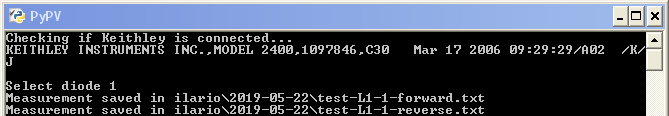
\includegraphics[width=1\textwidth]{PyPV/pypv-console.png}
 				\subcaption{Console output}\label{fig:pypv-console}
 			\end{subfigure}
 			\qquad
 			\begin{subfigure}[t]{0.41\textwidth}
 				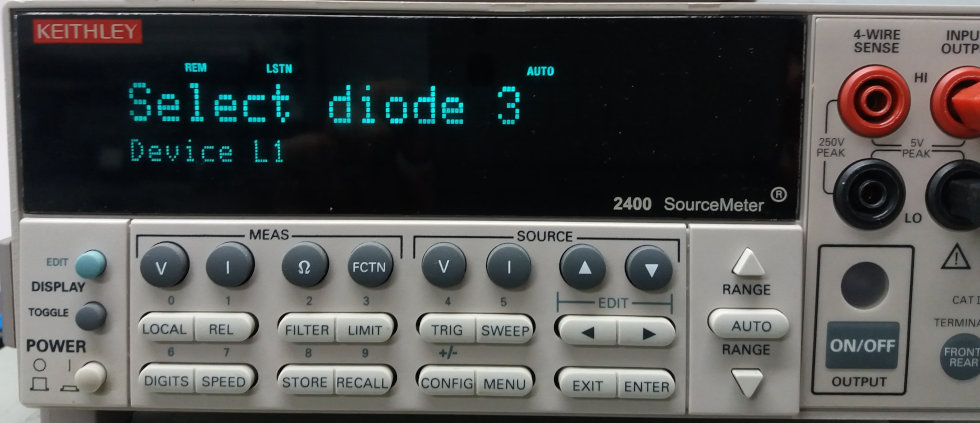
\includegraphics[width=1\textwidth]{PyPV/keithley.jpg}
 				\subcaption{Keithley display output}\label{fig:pypv-keithley}
 			\end{subfigure}
 			\mycaption[Additional output of PyPV\@.]{In (\textbf{a}) the textual output from console is shown.
 				The printed information is usually not important for normal software usage but can help for debugging.
 				In (\textbf{b}) instructions to the user are delivered \textsl{via} Keithley's display and buzzer.
 			}\label{fig:pypv-other}
 		}
 	}
 \end{figure}
 
\paragraph{Additional output}
Python console in \cref{fig:pypv-console} is used mainly for reporting additional data \textsl{e.g.}\ where the files got saved or each of the measured steady state \gls{voc} points.
Keithley's display in \cref{fig:pypv-keithley} is used for communicating to the user which diode has to be measured during the "AutoMeasure".
Moreover, the same information is also outputted using Keithley's buzzer as a number of beeps.

\subsection{Output files}
	
\paragraph{Directories naming}\label{pypv_naming_directories}
When using the "AutoSave" of the "AutoMeasure" functions, the following directory structure is created, if not already existing: \texttt{user name\-/YYYY-MM-DD} where the subdirectory is the measurement date in little endian format.

\paragraph{Files naming}\label{pypv_naming_files}
When using the "AutoSave" of the "AutoMeasure" functions, inside the aforementioned directory the measurements are named with the following schema: \texttt{experiment name-device name-\textit{<diode>}-\textit{<direction>}.txt} where \textit{\texttt{<diode>}} is the identification number of the specific diode under measurement, in case there is more than one per substrate (\textsl{e.g.}\ in our case, each device has four independent diodes, as can be seen in \cref{fig:device}) and \texttt{\textit{<direction>}} can be either \texttt{forward} or \texttt{reverse}, as explained in \cpageref{characterization_fwdrev} for the sweep scan direction.
In case an illumination different from \SI{100}{\mW\per\square\cm} was used, a field is added specifying it in the file name.
For example, a typical path and file name could be: \texttt{ilario/\-2019-06-18/\-ig79-c26-2-0.25sun-reverse.txt}.
In order to improve the compatibility with different file systems, the accents in the user name, experiment name, and device name fields are removed using \texttt{unicode\-data.\-normalize} function.

\paragraph{Files content}
In the txt files, the first 22 lines include some information about: user, date and time, experiment name, device name, diode number, scan direction, lowest and highest sweep voltage, voltage step size, compliance (maximum current), scale, calculated voltage and current density of maximum power point, integration time and the related scan speed, delay time for each measured point, pre-delays for closed and opened illumination shutter, calculated series resistance (from the high voltage points) and shunt resistance (from close\hyp{}to\hyp{}zero voltage points), active area, irradiance (illumination intensity in \si{\mW\per\square\cm}), calculated \gls{jsc}, \gls{voc}, fill factor, and \gls{pce}.
The \nth{23} row include the header for the data.
From the \nth{24} row on, two columns with applied voltage and measured current follow, separated by a tabulation.
The rows are terminated by a \texttt{\n} newline, following the Unix standard.

\paragraph{Configuration saving}
Usually, the setup does not change between experiment and experiment.
To reduce the risk of setting wrongly some parameters, some of them are saved in the \texttt{last\_configuration.lnk} file at the program's closing and restored at its opening.
The parameters which get saved are: user name, experiment name, lower and higher voltages, voltage step size, compliance value, scale, integration time, and cell area.

\paragraph{Logging and recovery files}
The software execution dates and the main parameters of all the performed measurements are stored in a log file: \texttt{measurements\_log.txt}.
In case the user closes the software forgetting to save the last measurement, the data is also saved in two temporary files: \texttt{last\_measurement\_raw.txt} and \texttt{last\_measurement.txt} containing respectively the latest raw and processed measurement output.

	\subsection{Limitations}

		The interface development has been started with the "Monkey Studio" software, which development has ceased even before the start of PyPV\@.
		This demonstrated to be a failure in long term development planning.

%\pagebreak[2]
\newpage
\section{Robust and quick data analysis \textsl{via} R scripts}
	\epigraph{\textit{\enquote{Is there an Origin version for Linux?}\\\enquote{No}}}

	\subsection{Introduction}
		To process the large amount of data which can be obtained using multiple techniques during the characterisation of solar cells can be a very tedious and repetitive work.
		We developed routines for data processing and representation, like fittings, integrations and plots.
		I am describing the routines here in order to allow others to use and modify them.
		The described routines have been tested to work on Linux and Windows systems.
		All of the described functions can be downloaded from \url{https://github.com/ilario/photophysics-data-processing-R}.
		Just the scripts which are relevant for the data published in this thesis will be reported, while many others (\textsl{e.g.}\ parameter extraction from current\hyp{}voltage sweeps, statistics on the performance parameters, Tauc plot fitting, logarithmic smoothing of transient absorption spectroscopy data\dots) can be found online.

	\subsection{Helpers}
		\paragraph{\texttt{limits\_for\_graphics.R} -- Set graphical parameters}
		In this file I tried to centralize the parameters which should be edited by the user and will be used by the scripts.
		This is for avoiding the need to edit "hardcoded" values in the middle of complex scripts.
		The parameters which can be customized here are: device active area, limits for the axes, string to prepend to the file names, switch between raster or vector image output, resolution of raster images output, size of vector image output.

		\paragraph{\texttt{devices-\-identification.R} -- Define grouping of devices}
		The devices are labelled with an alphanumeric codename, which is not insightful at the time of categorizing them for a statistical analysis.
		In this file the samples codes are grouped depending on one or two characteristics.
		Up to now, this system is just employed by \texttt{iv-generate\_mydata\_with\_comments.R} for adding supplementary information to the extracted parameters and by \texttt{iv-\-generate\_statistics.R} for plotting the boxplots separating the samples by kind.

		\paragraph{\texttt{run-\-all-\-photophysics.R} -- Runs routine data analysis on one device's data}
		An extremely basic but multiplatform \gls{gui} has been implemented.
		Running it, the data folder gets prompted.
		By default, all the data analysis routinely performed in Palomares group is run.
		It can be edited to unselect the non-needed data analysis routines.
		
		\paragraph{\texttt{run-\-all-\-photophysics-\-comparisons.R} -- Plots comparisons between devices}
		This basic \gls{gui} prompts the user for the directories containing the data of each of the devices to be compared.
		Then it plots the characterisation data of all the selected devices in single plots, in order to help the visual comparison of the results.
		
		%\subsection{Photophysical Characterization \textsl{via} Optical and Electrical Transients}


	\subsection{Charge Extraction (\glsentryshort{ce})}\label{r_ce}
	For details on \acr{ce} technique, see \cpageref{characterization_ce}.

		\paragraph{\texttt{from\_ce\_to\_table.R} -- Converts CE output}
		The output from \acr{ce} measurement software is rather minimal, as it lacks the time column.
		This script generates a two column file output which is more convenient for plotting with other commonly employed software.
		It works both for the TPV and for the TPC outputs.
		
		\paragraph{\texttt{ce.R} -- Integrates CE transients directly}
		Subtracts a base line from the voltage profile (a line joining the first voltage points to the last ones, so it could result in a slightly tilted base line) and divides it by the known instrumental resistance of \SI{50}{\ohm} in order to obtain the current.
		Then it integrates the current profile over time starting from time zero, which is the moment when circuit gets closed but due to some delay induced by the transistors the current flows just a few tenths of microsecond after, as shown in \cref{fig:ce_noise-normal}.

		\paragraph{\texttt{ce-\-subtractDark.R} -- Integrates CE transients after subtracting a transformed noise profile}
		Uses a pure noise signal obtained for each sample from a measurement in dark (no extracted charge, just instrumental noise due to transistors closing/opening) for fitting the noise profile in the illuminated solutions.
		Then subtracts the transformed noise profile and integrates the result over time.
		See \cpageref{characterization_subtractDark} and \cref{fig:ce_noise-subtractDark} for a more complete description.
		
		\paragraph{\texttt{ce-\-integrateExp.R} -- Integrates a fit to CE transients}
		Determines the start of the \acr{ce} decay from the last zero before the voltage maximum, then fits the decay with an exponential function.
		The fit is performed using a robust fitting routine (as implemented in \texttt{robust\-base} \cite{Maechler2018}) in order to avoid the influence from the voltage rise points.
		The integral function of the fitted exponential function is plotted and its value at infinite time is taken for the extracted charge.
				See \cpageref{characterization_integrateExp} and \cref{fig:ce_noise-integrateExp} for a more complete description.
				
		\paragraph{\texttt{ce-\-from\_output\_to\_graph.R} -- Plots the extracted charge \textsl{versus} light bias}
		Plots the output of a series of extracted charges \textsl{versus} light bias voltages.
		Then it fits the trend using \cref{eq:ce_full}.
		
		\paragraph{\texttt{ce-\-from\_many\_output\_to\_graph.R} -- Compares between CE of various devices}
		Plots the charge \textsl{versus} light bias trends of all the devices' data in the current directory, like in \cref{fig:tae_photophysics-ce}.
		This is used for comparisons like the one in the right column of \cref{fig:ce_noise}.
		
%		\paragraph{\texttt{ce-time-many.R} -- Compares single CE transients of various devices}
%		\paragraph{\texttt{ce-with\_limits.R} -- Compares CE transients with RC decays}

	\subsection{Transient PhotoVoltage (\glsentryshort{tpv})}\label{r_tpv}
	For details on \acr{tpv} technique, see \cpageref{characterization_tpv}.
	
		\paragraph{\texttt{from\_tpv\_tpc\_to\_table.R} -- Converts CE output}
		Similarly to \texttt{from\_ce\_to\_table.R}, this converts the one column raw file to a two columns text file.

		\paragraph{\texttt{tpv.R} -- Fits TPV decays}
		This rather large routine fits the single \acr{tpv} decays.
		The following features can be activated or deactivated editing the script header:
		bi-exponential fitting, robust fitting \cite{Maechler2018}, save the plots to PNG or PDF files, plot all the data points or use a 2D histogram for reducing the overplotting problem (see \cref{fig:tpv_robust}), additionally plot with abscissa and/or ordinate axis in logarithmic scale, plot residuals, allow the fitting to match negative peaks.
		In order to successfully perform the bi-exponential fits using \cref{eq:tpv_biexp}, a good initial guess is provided at first and then, if convergence is not obtained, random initial guesses.
		If cases where this is not enough, some data points from the beginning of the decay (the most noisy part of the decay) are removed until when the fit converges.
		Additionally, the voltage increase value $\Delta V$ is also calculated here and will be used by \acr{dc} scripts, as explained in \cpageref{characterization_dc}.
		
%		
%				\paragraph{\texttt{tpv\_onlyDeltaV.R} -- Gets the voltage increase from TPV decays}
%				
		\paragraph{\texttt{tpv-\-from\_output\_to\_graph.R} -- Plots TPV lifetimes \textsl{versus} light bias}
		This script plots the lifetimes obtained from mono or bi exponential fits in \texttt{tpv.R} \textsl{versus} light bias voltage, like in \cref{fig:tpv}.
		Additionally, it fits the high voltage points using \cref{eq:tpv_tau_vs_intensity}.
%		
%\paragraph{\texttt{tpv-from\_output\_to\_graph-with\_limits.R} -- Compares lifetime with RC time}
%
		\paragraph{\texttt{tpv-\-from\_many\_output\_to\_graph.R} -- Compares between TPV of various devices}
		Similarly to the aforementioned \texttt{tpv-\-from\_output\_to\_graph.R} script, this plots the mono\hyp{}exponential lifetime \textsl{versus} light bias data for various devices in the same plot, allowing the user to make a graphical comparison.
%
	\subsection{Transient PhotoCurrent (\glsentryshort{tpc})}\label{r_tpc}
	For details on \acr{tpc} technique, see \cpageref{characterization_tpc}.

		\paragraph{\texttt{tpc.R} -- Integrates TPC transients}
		Similarly to what \texttt{ce.R} does for integrating the \acr{ce} voltage transient, also this script directly integrates the voltage transients \textsl{versus} time after subtracting a baseline, like in \cref{fig:tpc}.
		
%		\paragraph{\texttt{tpc-vs-tpv-vs-ce.R} -- Compares the single transients from various techniques}
%
%
	\subsection{Differential Capacitance (\glsentryshort{dc})}\label{r_dc}
	For details on \acr{dc} technique, see \cpageref{characterization_dc}.

		\paragraph{\texttt{dc-\-from\_output\_to\_graph.R} -- Calculates and plots capacitance and charge from DC}
		This script takes the photogenerated charge $\Delta n$ output from \texttt{tpc.R} and the voltage increase $\Delta V$ output from \texttt{tpv.R} and obtains the voltage dependent capacitance using \cref{eq:dc}.
		In case the values from different \acr{tpc} measures differs, for example due to the presence of background illumination, the first quartile of all the measured $\Delta n$ is used.
		The value of the geometric capacitance\index{geometric capacitance} is obtained fitting the capacitance using \cref{eq:dc_full} and then taking the $C_|g|$ parameter value.
		The chemical capacitance\index{chemical capacitance} profile is obtained subtracting $C_|g|$ to the calculated capacitance profile.
		The obtained capacitance \textsl{versus} light bias discrete profiles are converted to a continuous profile using R's \texttt{Vectorize} function and integrated over voltage (see \cref{eq:dc_charge}) for obtaining the excess charge \textsl{versus} light bias trends with or without geometric capacitance\index{geometric capacitance}.

%		
%		\paragraph{\texttt{cedc.R} -- Compares the charge \textsl{versus} light\hyp{}bias obtained from CE or DC}
%		
		\paragraph{\texttt{dc-from\_many\_output\_to\_graph\_capacitance.R} and \texttt{dc-\-from\_many\_output\_to\_graph\_charge.R} -- Compares between DC of various devices}
		The comparison of capacitance and charge from \acr{dc} is plotted for various devices and fitted using \cref{eq:dc_full}, like in \cref{fig:dc_deltaV}.
		The data to be plotted is taken from the output of \texttt{dc-\-from\_output\_to\_graph.R} script.

	\subsection{Transient PhotoVoltage referred to charge from CE or DC (\glsentryshort{tpvce} and \glsentryshort{tpvdc})}\label{r_tpvcedc}
		For details on \acr{tpv}-CE and \acr{tpv}-DC techniques, see \cpageref{characterization_tpvce}.
%
%
%
%		\paragraph{\texttt{tpvce-from\_output\_to\_graph.R} -- Relate TPV lifetimes to CE charge}
		
				\paragraph{\texttt{tpvce-\-from\_many\_output\_to\_graph.R} and \texttt{tpvdc-\-from\_many\_output\_to\_graph.R} -- Compare TPV lifetimes related to either CE or DC charge of various devices}
The mono\hyp{}exponential lifetimes from \texttt{tpv.R} are plotted \textsl{versus} various charge profiles obtained from \acr{ce} or \acr{dc}.
In order to squash the light bias axes from the different techniques, the \acr{ce} or \acr{dc} charge \textsl{versus} voltage profiles are fitted and the employed charge value at the \acr{tpv} light biases is obtained from the fit.
The charge profiles employed are: complete charge including geometric capacitance\index{geometric capacitance}, chemical charge subtracting $C_|g|$ obtained either with \cref{eq:ce_full} for \acr{ce} or with \cref{eq:dc_full} for \acr{dc}.
Fitting the small perturbation lifetimes \textsl{versus} chemical charge using \cref{eq:tau_pfo}, the recombination order $\Phi$ is obtained.
This $\Phi$ is used for correcting the small perturbation lifetimes to total carrier lifetimes (pseudo first order lifetimes) using \cref{eq:tau_pfo} and is plotted again \textsl{versus} chemical charge.
An example of all the mentioned plots can be observed in \cref{fig:tpvce,fig:tae_photophysics_tpvcedc}.

%	\subsection{Current-Voltage Sweeps}
%		\paragraph{\texttt{extractdata-curves-vi-separated\_files.R} -- Functions for extracting parameters from current\hyp{}voltage sweeps¨}
%		\paragraph{\texttt{iv-generate\_mydata.R} and \texttt{iv-generate\_mydata\_with\_comments.R}}
%		\paragraph{\texttt{iv-generate\_images.R}}
%				\paragraph{\texttt{iv-plot\_list.R}, \texttt{iv-plot\_list-suppinfo.R}, and \texttt{iv-light\_intensity.R}}
%		\paragraph{\texttt{iv-generate\_statistics.R}}
%		\paragraph{\texttt{iv-jsc\_voc\_vs\_light\_intensity.R}}

%
%		\paragraph{\texttt{jsc-stability.R} and \texttt{voc-stability.R}}
%
%	\subsection{Other}
%	Not all the scripts are described in this chapter, two of the most interesting others will be reported here:
%	
%				\paragraph{\texttt{jrec-ce.R} and \texttt{jrec-dc.R} -- Reconstructs the \gls{jsc}}
%					\cpageref{jsc_reconstruction}
%					
%		\paragraph{\texttt{mppt\_to\_graph.R} -- Plots tracking of maximum power point}
%		\paragraph{\texttt{profilometry.R} -- Plots profilometer measurements and fit heights}
%		\paragraph{\texttt{tas-downsample.R} -- Reduces the dimension of TAS decays}
%%		\paragraph{\texttt{tas-graph.R} -- Plots TAS decays}
%		\paragraph{\texttt{uvvis-pl.R} -- Plots absorbance and photoluminescence spectra and fits Tauc plots}

\newpage
\section{Contributions to mppTracker}\label{software_mppt}
	\epigraph{\textit{\enquote{A student of mine sells a complete system for that, just go and buy it}}}
	

	As seen in \cpageref{characterization_hysteresis}, a \acr{mppt} system ensures to obtain a \gls{pce} value closer to the real world working conditions \cite{Zimmermann2016}.
	The hysteretic\index{hysteresis} phenomena in perovskite solar cells requires new procedures for \acr{mppt} \cite{Cimaroli2017,Pellet2017,Rakocevic2019} and a few commercial systems are already available for that \cite{CicciResearchsrl2019,CandlelightSystems}.
	An interesting project for having robust \acr{mppt} measurable with Tektronix Keithley 2400 is mppTracker \cite{AFMD2017}.
	I made a few contributions which are accessible on \url{https://github.com/AFMD/mppTracker/pulls?q=is%3Apr}.
	As the effort in this project were very limited on my side, I will not further describe that but an example of the output is reported in \cref{fig:mppt}.
	If confirmed, recent reports on "bistable short circuit current" in perovskite solar cells by \authoryear{Calado2018} would further complicate the implementation of a \acr{mppt}.
	\begin{figure}[H]
			\makebox[\textwidth][c]{
			\parbox{1.1\textwidth}{
		\centering
		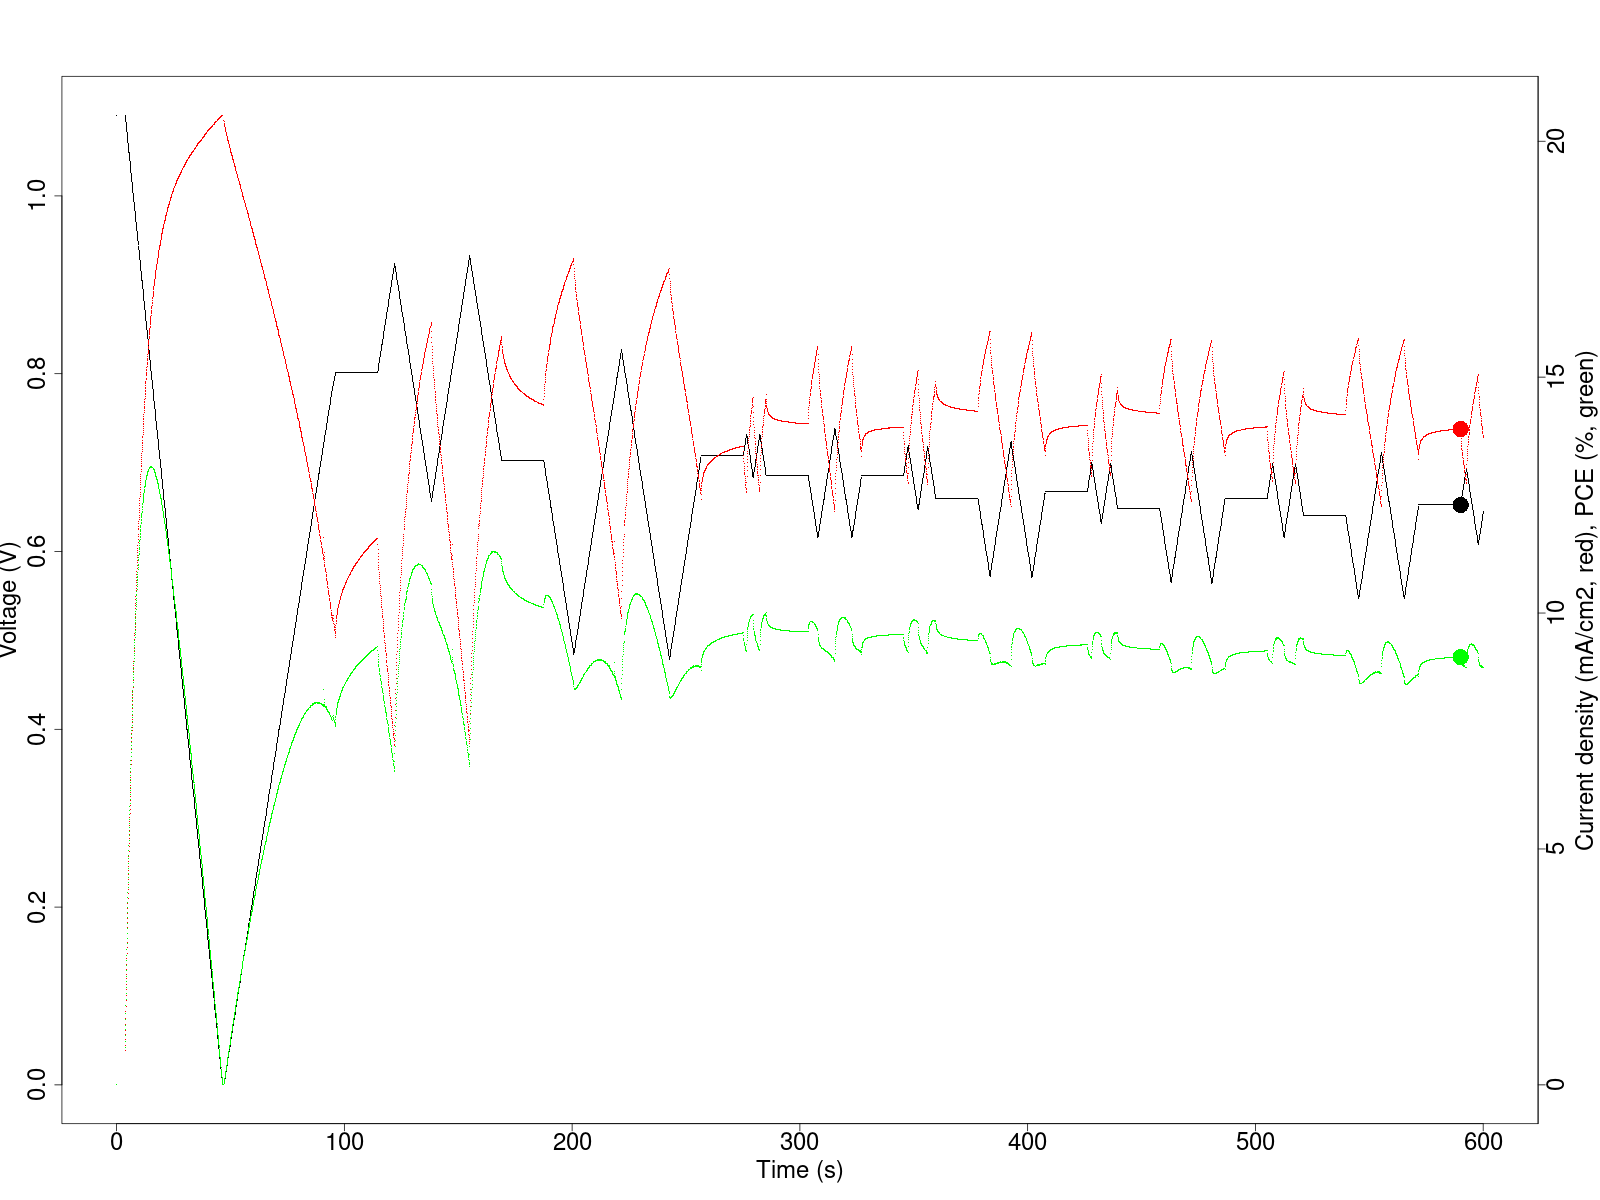
\includegraphics[width=0.9\textwidth]{mppt/ig92-spiro-1456-1-led437penta.png}
		\mycaption[Example of maximum power tracking measurement.]{
			A perovskite solar cell has been measured with an improved version of mppTracker.
			The black line is the applied voltage and refers to the left axis.
			The red line is the measured current and refers to the right axis.
			Te resulting \gls{pce} is the green line and is also on the right axis.
		}\label{fig:mppt}
	}}
	\end{figure}

%	\begin{minipage}{\linewidth}
%		\begin{center}
%	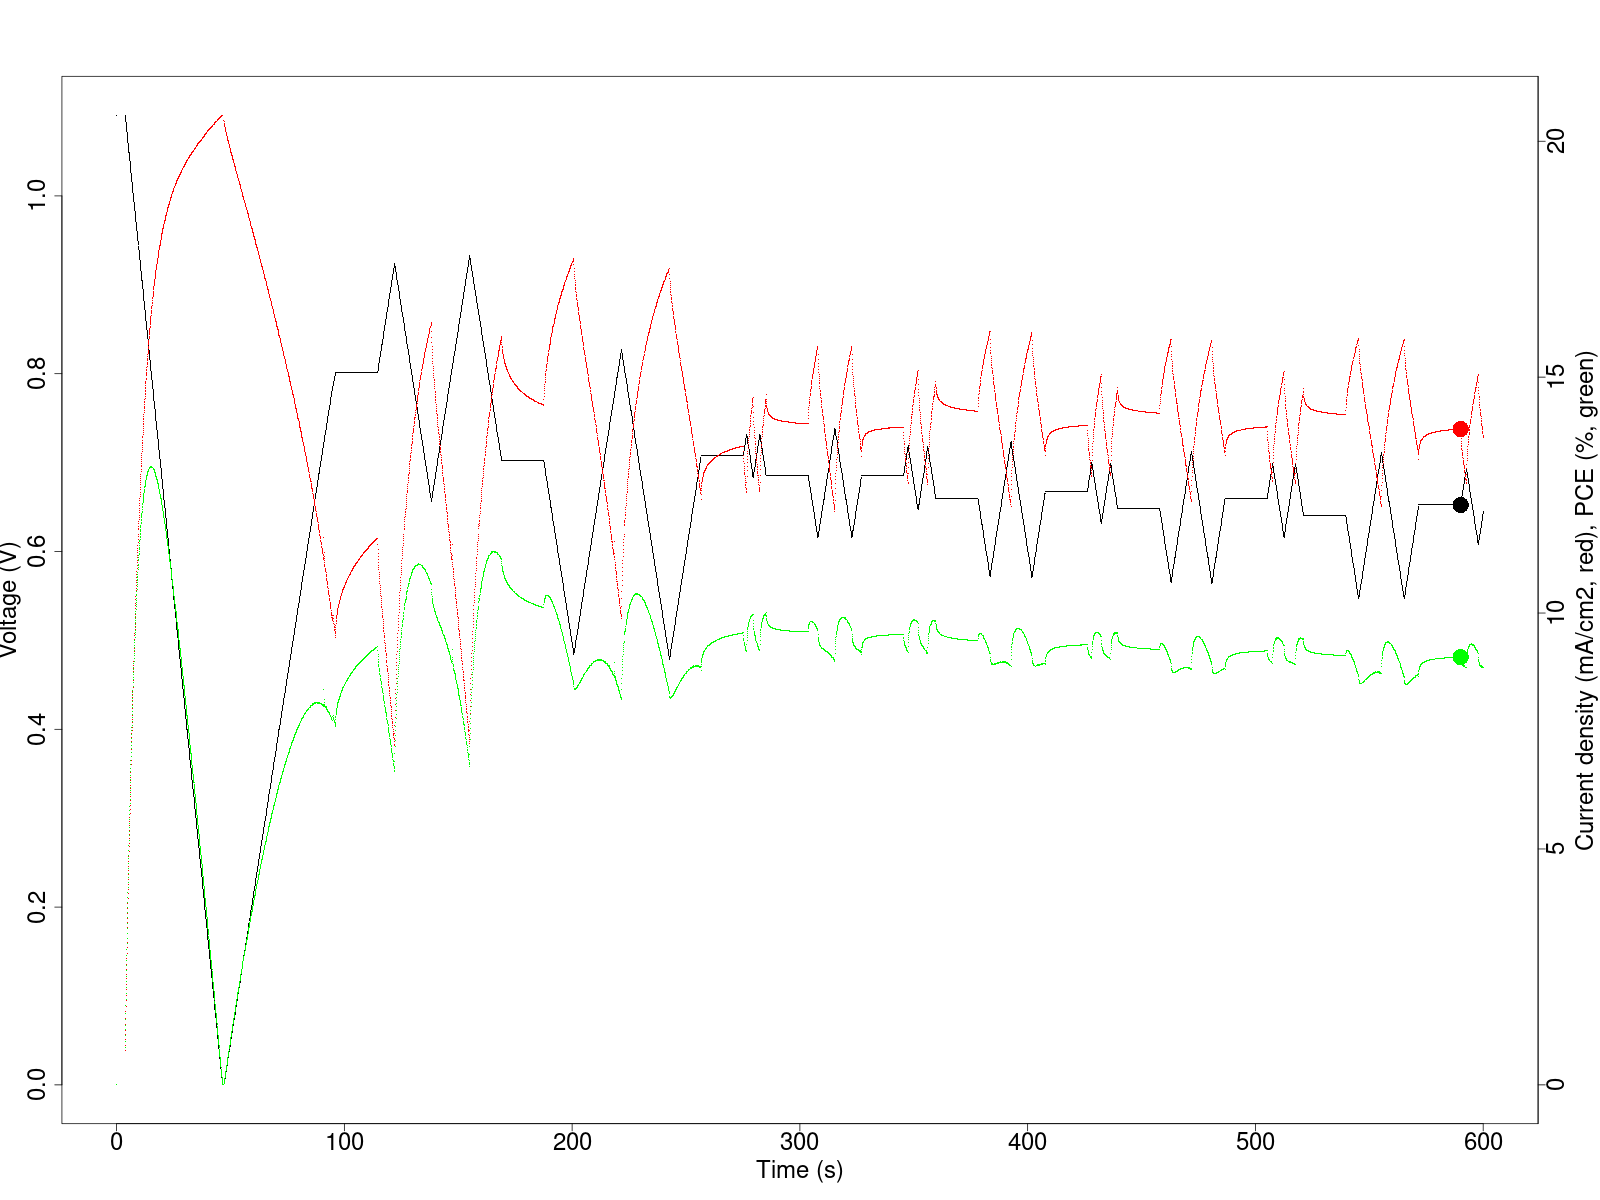
\includegraphics[width=1\textwidth]{mppt/ig92-spiro-1456-1-led437penta.png}
%			\captionof{figure}[Example of maximum power tracking measurement.]{\textbf{Example of maximum power tracking measurement.}
%					The reported measurement has been performed with an improved version of mppTracker on a \gls{fto}\-/\ch{d-TiO2}\-/\gls{csfamapbibr}\-/\gls{spiro}\-/\ch{Au} solar cell.
%			The black line indicates the applied voltage and refers to the left axis.
%			The red line represents the measured current and refers to the right axis.
%			Te resulting power conversion efficiency is the green line and is also on the right axis.
%		}\label{fig:mppt}
%		\end{center}
%	\end{minipage}
	


